\section{双曲函数、反双曲函数}
\begin{definition}[双曲函数]
\begin{gather}
	\sinh x \defeq \frac{e^x - e^{-x}}{2}. \\
	\cosh x \defeq \frac{e^x + e^{-x}}{2}. \\
	\tanh x \defeq \frac{\sinh x}{\cosh x} = \frac{e^x - e^{-x}}{e^x + e^{-x}}. \\
	\coth x \defeq \frac{1}{\tanh x} = \frac{e^x + e^{-x}}{e^x - e^{-x}}.
\end{gather}
这里,
\(\sinh x\)被称为\DefineConcept{双曲正弦},
\(\cosh x\)被称为\DefineConcept{双曲余弦},
\(\tanh x\)被称为\DefineConcept{双曲正切},
\(\coth x\)被称为\DefineConcept{双曲余切}.
\end{definition}

\begin{figure}[ht]
	\centering
	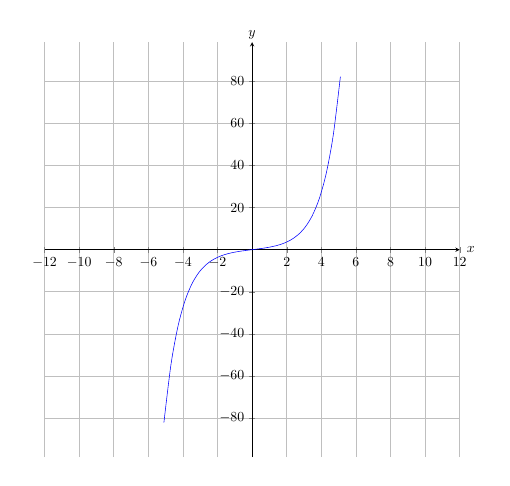
\begin{tikzpicture}[scale=.5]
		\begin{axis}[
			xmin=-10,xmax=10,
			restrict y to domain=-100:100,
			grid=both,width=\textwidth,height=\textwidth,
			axis lines=middle,
			xlabel={\(x\)},
			ylabel={\(y\)},
			enlarge x limits=0.1,
			enlarge y limits=0.1,
			x label style={at={(ticklabel* cs:1.00)}, inner sep=5pt, anchor=west},
			y label style={at={(ticklabel* cs:1.00)}, inner sep=2pt, anchor=south},
		]
			\addplot[color=blue,samples=50,smooth,domain=-10:10]{.5*(exp(x)-exp(-x))};
		\end{axis}
	\end{tikzpicture}
	\caption{双曲正弦函数的图形}
	\label{figure:函数.双曲正弦函数的图形}
\end{figure}

\begin{figure}[ht]
	\centering
	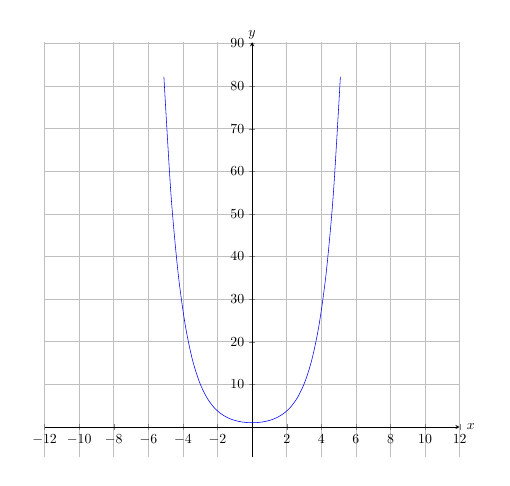
\begin{tikzpicture}[scale=.5]
		\begin{axis}[
			xmin=-10,xmax=10,
			restrict y to domain=-100:100,
			grid=both,width=\textwidth,height=\textwidth,
			axis lines=middle,
			xlabel={\(x\)},
			ylabel={\(y\)},
			enlarge x limits=0.1,
			enlarge y limits=0.1,
			x label style={at={(ticklabel* cs:1.00)}, inner sep=5pt, anchor=west},
			y label style={at={(ticklabel* cs:1.00)}, inner sep=2pt, anchor=south},
		]
			\addplot[color=blue,samples=50,smooth,domain=-10:10]{.5*(exp(x)+exp(-x))};
		\end{axis}
	\end{tikzpicture}
	\caption{双曲余弦函数的图形}
	\label{figure:函数.双曲余弦函数的图形}
\end{figure}

\begin{figure}[ht]
	\centering
	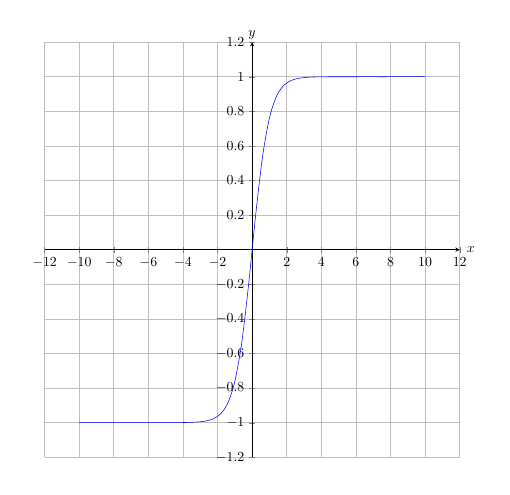
\begin{tikzpicture}[scale=.5]
		\begin{axis}[
			xmin=-10,xmax=10,
			restrict y to domain=-100:100,
			grid=both,width=\textwidth,height=\textwidth,
			axis lines=middle,
			xlabel={\(x\)},
			ylabel={\(y\)},
			enlarge x limits=0.1,
			enlarge y limits=0.1,
			x label style={at={(ticklabel* cs:1.00)}, inner sep=5pt, anchor=west},
			y label style={at={(ticklabel* cs:1.00)}, inner sep=2pt, anchor=south},
		]
			\addplot[color=blue,samples=50,smooth,domain=-10:10]{(exp(x)-exp(-x))/(exp(x)+exp(-x))};
		\end{axis}
	\end{tikzpicture}
	\caption{双曲正切函数的图形}
	\label{figure:函数.双曲正切函数的图形}
\end{figure}

\begin{figure}[ht]
	\centering
	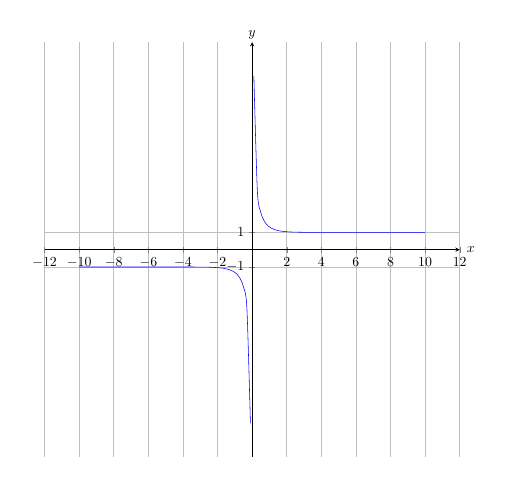
\begin{tikzpicture}[scale=.5]
		\begin{axis}[
			xmin=-10,xmax=10,
			ymin=-10,ymax=10,
			grid=both,width=\textwidth,height=\textwidth,
			axis lines=middle,
			xlabel={\(x\)},
			ylabel={\(y\)},
			enlarge x limits=0.1,
			enlarge y limits=0.1,
			x label style={at={(ticklabel* cs:1.00)}, inner sep=5pt, anchor=west},
			y label style={at={(ticklabel* cs:1.00)}, inner sep=2pt, anchor=south},
			ytick={-1,1},
		]
			\addplot[color=blue,samples=50,smooth,domain=-10:-.1]
				{(exp(x)+exp(-x))/(exp(x)-exp(-x))};
			\addplot[color=blue,samples=50,smooth,domain=.1:10]
				{(exp(x)+exp(-x))/(exp(x)-exp(-x))};
		\end{axis}
	\end{tikzpicture}
	\caption{双曲余切函数\(y=\coth x\)的图形}
	\label{figure:函数.双曲余切函数的图形}
\end{figure}

下面我们研究双曲函数的反函数.

首先讨论双曲正弦\(y=\sinh x\)的反函数.
由\(x=\sinh y\),有\[
	x=\frac{e^y-e^{-y}}{2}.
\]
令\(u=e^y\),则有\[
	u^2-2xu-1=0.
\]
这是一个关于\(u\)的一元二次方程,解得\[
	u=x\pm\sqrt{x^2+1}.
\]
因为\(u=e^y>0\),故上式根号前应取正号,即\[
	u=x+\sqrt{x^2+1}.
\]
又由\(y=\ln u\),故得反双曲正弦\[
	\arsinh x
	\defeq
	\ln(x+\sqrt{x^2+1}),
	\quad -\infty<x<+\infty.
\]

接下来讨论双曲余项\(y=\cosh x\)的反函数.
由\(x=\cosh y\),有\[
	x=\frac{e^y+e^{-y}}{2}, \quad y\geq0.
\]
由此得\(e^y=x\pm\sqrt{x^2-1}\),
故\[
	y=\ln(x\pm\sqrt{x^2-1}).
\]
上式中\(x\)的取值必须满足条件\(x\geq1\),
而其中平方根前的符号由于\(y\geq0\)而应取正号,
故\[
	y=\ln(x+\sqrt{x^2-1}).
\]
上述双曲余弦\(y=\cosh x\ (x\geq0)\)的反函数称为反双曲余弦的主值,
记作\(\arcosh x\),
即\[
	\arcosh x
	\defeq
	\ln(x - \sqrt{x^2 - 1}),
	\quad 1\leq x<+\infty.
\]

类似地可得反双曲正切\[
	\artanh x
	\defeq
	\frac{1}{2} \ln\frac{1 + x}{1 - x},
	\quad -1<x<1;
\]
以及反双曲余切\[
	\arcoth x
	\defeq
	\frac{1}{2} \ln\frac{x + 1}{x - 1},
	\quad -\infty<x<-1\lor1<x<+\infty.
\]

\begin{property}
\(\sinh x\)是奇函数,即对\(\forall x \in [-a,a]\)有\[
	\sinh(-x) = -\sinh x;
\]

\(\cosh x\)是偶函数,即对\(\forall x \in [-a,a]\)有\[
	\cosh(-x) = \cosh x.
\]
\end{property}

\begin{property}
\(\cosh x\)有下界:\[
	\cosh x \geq 1
\]
当且仅当\(x=0\)时,上式取等号.
\end{property}

\begin{theorem}
\begin{gather}
	\sinh(x \pm y) = \sinh x\cosh y \pm \cosh x\sinh y, \\
	\cosh(x \pm y) = \cosh x\cosh y \pm \sinh x\sinh y, \\
	\tanh(x + y) = \frac{\tanh x + \tanh y}{1 + \tanh x\tanh y}.
\end{gather}
\begin{proof}
根据双曲函数的定义有
\begin{align*}
	\sinh x\cosh y+\cosh x\sinh y
	&= \frac{e^x - e^{-x}}{2} \frac{e^y + e^{-y}}{2}
		+ \frac{e^x + e^{-x}}{2} \frac{e^y - e^{-y}}{2} \\
	&= \frac{1}{4} (e^x e^y + e^x e^{-y} - e^{-x} e^y - e^{-x} e^{-y} \\
	&\qquad+ e^x e^y - e^x e^{-y} + e^{-x} e^y - e^{-x} e^{-y}) \\
	&= \frac{1}{4} (2 e^x e^y - 2 e^{-x} e^{-y}) \\
	&= \frac{1}{2} (e^{x+y} - e^{-x-y}) = \sinh(x+y).
\end{align*}
\begin{align*}
	\cosh x\cosh y+\sinh x\sinh y
	&= \frac{e^x + e^{-1}}{2} \frac{e^y + e^{-y}}{2}
		+ \frac{e^x - e^{-x}}{2} \frac{e^y - e^{-y}}{2} \\
	&= \frac{1}{4} (e^x e^y + e^x e^{-y} + e^{-x} e^y + e^{-x} e^{-y} \\
	&\qquad+ e^x e^y - e^x e^{-y} - e^{-x} e^y + e^{-x} e^{-y}) \\
	&= \frac{1}{4} (2 e^x e^y + 2 e^{-x} e^{-y}) \\
	&= \frac{1}{2} (e^{x+y} + e^{-x-y}) = \cosh(x+y).
	\qedhere
\end{align*}
\end{proof}
\end{theorem}

\begin{theorem}
\begin{gather}
	\cosh^2x - \sinh^2x = 1, \\
	\sinh x + \cosh x = e^x, \\
	\cosh x - \sinh x = e^{-x}, \\
	1 - \tanh^2{x} = \frac{1}{\cosh^2x}, \\
	\coth^2{x} - 1 = \frac{1}{\sinh^2x}.
\end{gather}
\begin{proof}
根据双曲函数的定义有
\begin{align*}
	\cosh^2x-\sinh^2x
	&=\left(\frac{e^x + e^{-x}}{2}\right)^2-\left(\frac{e^x - e^{-x}}{2}\right)^2 \\
	&=\frac{e^{2x}+2+e^{-2x}}{4}-\frac{e^{2x}-2+e^{-2x}}{4}
	=1.
	\qedhere
\end{align*}
\end{proof}
\end{theorem}

\begin{theorem}
\begin{gather}
	\sinh2x = 2 \sinh x\cosh x, \\
	\cosh2x = \cosh^2x + \sinh^2x.
\end{gather}
\end{theorem}
